\chapter{Concept}\label{chap:Concept}

\section{The type system}\label{sec:concept:TypeSystem}

In \ref{subsec:background:TypeSystems}, we introduce the concept of type systems and we give a brief overview of \textit{type checking} and \textit{type inference}. Our goal is to have solid \textit{application programming interfaces} (APIs) to build type systems for each language.
In this section, we will discuss the importance of the type system for our concept.
What we are looking for in our type system is:
\begin{itemize}
    \item \textbf{modularization}, that allows the definition of custom types and operations on these types, and the ability to combine them in a modular way;
    \item \textbf{flexibility}, since the type system is not known \textit{a priori}, we need the ability to adapt the type system to the specific needs;
    \item \textbf{easy-to-use}, extending the default implementation of the type system with a new type, or implementing a new type from scratch should be easy and straightforward.
\end{itemize}

It is trivial to remember that the type system should also provide the basic functionalities of a type system, such as \textbf{type inference}, that allows the compiler to infer the type of an expression without the need to explicitly specify it; and \textbf{type checking}, that allows the compiler to check if the types of the expressions are correct.

\subsection{The relevance of the type system in the LSP design}\label{subsec:concept:RelevanceOfTheTypeSystem}

The type system is the core of the LSP design. We illustrate the need of having a type system by focusing on the ability to respond to requests from a \textit{Language Client}.

In the reminder of this section, we will evaulate the relevance for three of the most important LSP feautre introduced in \ref{subsec:bacground:KeyMethodsOverview}.

\subsubsection{Diagnostic Analysis}\label{subsubsec:concept:DiagnosticAnalysis}

Currently, the LSP provides the ability to perform \textit{diagnostic analysis} on the code. This feature is useful to provide feedback to the user about the correctness of the code.
In compilers design, a \textit{Diagnostic} can be produced by different phases of compilation, such as the \textit{lexical analysis}, \textit{syntax analysis}, and \textit{semantic analysis}.
The \textbf{Syntax Errors} are detected by the \textit{lexical analysis} and \textit{syntax analysis}, usually during the \textit{parsing} phase. The \textbf{Semantic Errors} are detected by the \textit{semantic analysis}, usually during the \textit{type checking} phase.
In modern compilers, an additional phases can be added to the compilation process, \textit{data flow analysis} and \textit{control flow analysis}, that can be used to detect more complex errors, such as \textit{unreachable code} or \textit{dead code}.

In Language Workbenches world, usually it is common to have an instance of a \textbf{Language} and a \textbf{Source Code} that should be parsed and analyzed by the Language.
Taking into account the \textbf{Syntax Errors}, assuming that the \textbf{Language} is able to parse the \textbf{Source Code} and the \textbf{Language} is able to provide errors and warnings during the \textit{parsing} phase, should be easy to provide the \textit{Syntax Errors} to the \textit{Language Client} (see Listing \ref{lst:concept:SyntaxError}).

\begin{Listing}[t]
    \centering
    \showjava*[1\textwidth]{SyntaxError.java}
    \caption{Example of catching a Syntax Error in Java}
    \label{lst:concept:SyntaxError}
\end{Listing}

The \textbf{Semantic Errors} and \textbf{Data Flow Analysis} are more complex to implement. In fact, in order to detect a \textit{Semantic Error}, the \textbf{Language} should be able to perform \textit{type checking} on the \textbf{Source Code} in order to verify that the code can be executed without any unexpected errors. The \textit{Data Flow Analysis} is necessary to understand if the code is reachable, and to do this, the \textbf{Language} should be able to perform static analysis on the \textbf{Source Code}.

\subsubsection{Jump to Definition}\label{subsubsec:concept:JumpToDefinition}
The ability to access the definition of a symbol, such as a function or a variable, is a common feature in modern IDEs.
To enable this functionality, a \textbf{Symbol Table} is required and should be able to map a given row and column position in the source code to the corresponding symbol and its definition.
During this phase, the typechecking is required to bind the symbol to its type. This is necessary to provide the correct definition of the symbol to the user.
In addition to the symbol table, the \textbf{Language} should be able to provide the \textit{Scope} of the symbol, in order to understand if the symbol is visible in the current context.

\subsubsection{Code Completion}\label{subsubsec:concept:CodeCompletion}

To effectively handle this kind of request, such as the one depicted in figure~\ref{fig:completion}, the language server needs to comprehend the type of symbol for which suggestions are to be provided. Once the type is determined, returning relevant suggestions becomes straightforward. However, a challenge arises when suggestions must be presented to the user while they are still writing, as the source code may be syntactically incorrect during the writing process. To address this issue, a parser with error detection and recovery~\cite{Graham79} capabilities is required to enable effective suggestion generation despite the presence of syntax errors.

\section{Towards a modular type system}\label{sec:concept:TowardsAModularTypeSystem}

In this section, we will discuss the importance of having a modular type system for the LSP design. In particular, we will focus on the ability to define custom types and operations on these types, and the ability to combine them in a modular way.

\begin{mydefinition}{Type system item}{concept:itemdefinition}
  % This is the text of the theorem. The counter is automatically assigned and,
  % in this example, prefixed with the section number. This theorem is numbered with
  %   \ref{def:concept:itemdefinition} and is given on page \pageref{def:concept:itemdefinition}.
    Given that the specifics of the target language for the reference type system are not predetermined (i.e., the language is not known \textit{a priori}), we cannot assume the presence of standard programming constructs such as variables, functions, or objects. Therefore, to maintain a broad and adaptable approach, we will use the term \textbf{item} to refer to any of these potential constructs or elements within the system. This ensures that our discussion remains relevant regardless of the particular features and paradigms of the target language.
\end{mydefinition}

\subsection{Type: the basic building block}\label{subsec:concept:TypeTheBasicBuildingBlock}

The \textbf{Type} is the basic building block of the type system. It is used to represent the type of an expression, such as a variable, a function, or an object. The \textbf{Type} can be a primitive type, such as \textit{int}, \textit{float}, \textit{string} or a custom type, such as a \textit{class}, \textit{interface}, or \textit{enum}.

\begin{mydefinition}{Type}{concept:type}
The name \textbf{type} could be misleading because it does not exactly represent the type of an item but rather it is class of types that allows to build a specific type of a given category. Note that, this is not excluing that each concreate type could have a specific (class of) \textbf{type}, but defining a \textbf{type} as a class of types allows to define a generic \textbf{type} for all the types of a given category (i.e., all primitive types) and defining once the operations that can be performed on them.
\end{mydefinition}

In our concept, during the implementation of the type system, several types will be defined. Each type will have a set of operations that can be performed on it. In abstract terms, we can define a type as a set of operations that can be performed on it.
Basically, each type should be answer to the following questions:
\begin{enumerate}
    \item What is its \textbf{identifier}?
    \item Can it be \textbf{assignable from} another type with a specific kind of \textbf{variance}?
    \item Can it match a specific \textbf{signature}?
\end{enumerate}

The second question is used to \textbf{type check} the \textit{item} in the \textbf{Type System}. The type of \textbf{variance} is used to define the relationship between two types. The variance can be \textit{covariant}, \textit{contravariant}, or \textit{invariant}.

\begin{definition}{Variance}\\
    Suppose $A$ and $B$ are types, and $I[U]$ denotes application of a type constructor I with type argument $U$. Within the type system of a programming language, a typing rule for a type constructor $I$ is:
    \begin{itemize}
        \item covariant if it preserves the ordering of types ($\leq$), which orders types from more specific to more generic: If $A \leq B$, then $I[A] \leq I[B]$;
        \item contravariant if it reverses this ordering: If $A \leq B$, then $I[B] \leq I[A]$;
        \item bivariant if both of these apply (i.e., if $A \leq B$, then $I[A] \equiv I[B]$);
        \item variant if covariant, contravariant or bivariant;
        \item invariant or nonvariant if not variant.
    \end{itemize}
\end{definition}

The third question is used to \textbf{type inference} the \textit{item} in the \textbf{Type System}, simply answering to the question: can the type of the \textit{item} match a specific \textbf{signature}?


\subsection{Scope: the context of the type}\label{subsec:concept:ScopeTheContextOfTheType}


\begin{mydefinition}{Scope}{concept:scope}
The \textbf{Scope} is the context in which the type is defined, more precisely, where the binding between the type and the item is defined in the \textbf{Type System}. It is used to define the visibility and the lifetime of the type and its operations. The \textbf{Scope} can be, for example, a \textit{local scope}, a \textit{global scope}, or a \textit{module scope}.
\end{mydefinition}



\section{Modular implementation of LSP and DAP}\label{sec:concept:ModularImplementationOfLSPAndDAP}

\begin{figure}[t]
    \centering
    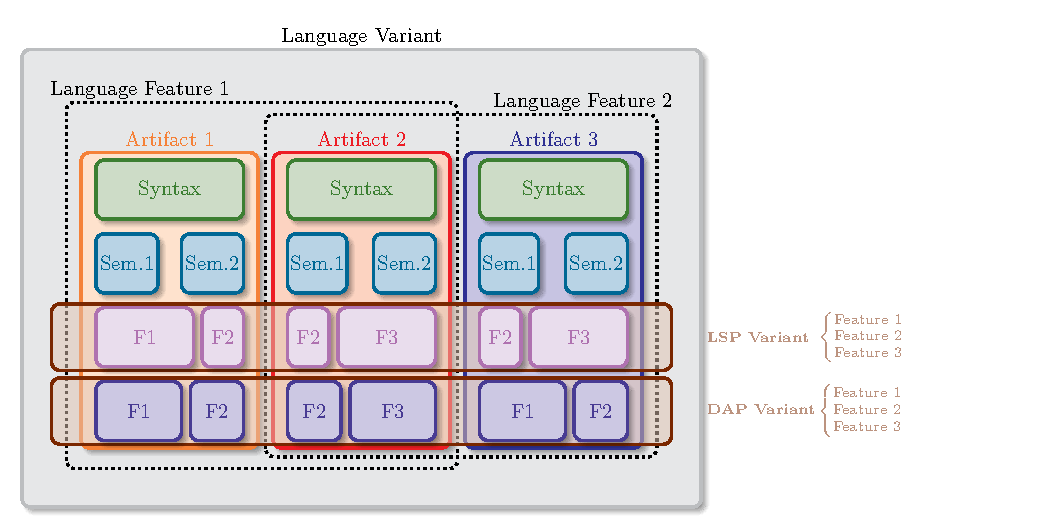
\includegraphics[width=0.9\linewidth]{figs/concept/module_with_lsp.pdf}
    \caption{Proposed approach to modular implementation of LSP and DAP.}
    \label{lst:concept:module_with_lsp}
\end{figure}


\section{Reduce to $\mathcal{L} \times 1$ the number of combinations to support $\mathcal{L}$ languages}

\begin{figure}[t]
    \centering
    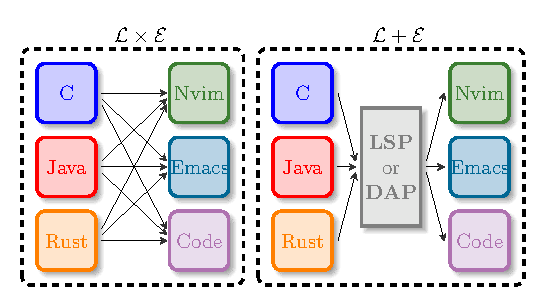
\includegraphics[width=0.9\linewidth]{figs/concept/lsp_combinations.pdf}
    \caption{Traditional approach vs LSP/DAP approach to language support.}
    \label{lst:conept:lsp_combinations}
\end{figure}

